\documentclass[tikz,border=10pt]{standalone}
\usepackage{tikz}
\begin{document}
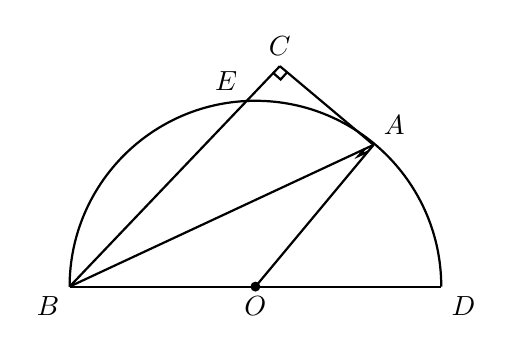
\begin{tikzpicture}[scale=1, line width=0.8pt]
  % points
  \coordinate (O) at (0,0);
  \coordinate (B) at (-2.36,0);
  \coordinate (D) at (2.36,0);
  \coordinate (A) at (1.5,1.8);
  \coordinate (C) at (0.31,2.8);
  \coordinate (E) at (-0.1,2.36);

  % semicircle
  \draw (B) arc (180:0:2.36);

  % base diameter
  \draw (B) -- (D);

  % segments
  \draw (B) -- (A);
  \draw (A) -- (O);
  \draw (B) -- (C);
  \draw (C) -- (A);

  % right angle mark at C
  \draw (0.23,2.71) -- (0.32,2.63) -- (0.40,2.72);

  % right angle mark at A
  \draw (1.39,1.75) -- (1.31,1.66) -- (1.42,1.71);

  % points
  \fill (O) circle (1.8pt);

  % labels
  \node[below left] at (B) {$B$};
  \node[below] at (O) {$O$};
  \node[below right] at (D) {$D$};
  \node[above right] at (A) {$A$};
  \node[above] at (C) {$C$};
  \node[above left] at (E) {$E$};
\end{tikzpicture}
\end{document}
